\chapter{Vibrations and Noise}
Vibrations are of great concern in the development of quadrotor flight controllers, and even more so when introducing variable pitch. The addition of variable pitch mechanisms increases the mechanical complexity of the quadrotor by adding more moving parts, thus creating more sources of vibrations.
\\
\\
On a quadrotor, the four individual motors generate vibrations which are carried through the frame and affects stabilization by disturbing the readings of the inertial measuring unit. If vibrations become to severe, stabilization will be difficult to achieve.
\\
\\
Bench testing shows that the vibrations increase significantly when the variable pitch mechanisms are attached to the motors. Therefore, it is important that all other sources of vibrations are minimized as much as possible. The frame, holes, parts and mechanical linkages therefore have to be as made as precise as possible. 
\\
\\
The commercial variable pitch mechanisms used in this project does also show imperfections. On high RPM, the inner shaft vibrates uncontrollably resulting in major disturbances in the IMU.
\\ 
\\
In order to minimize the vibration issues, counter measures must be taken. There are several ways of reducing vibrations and noise, mechanical, electrical and software counter measures can be taken. 
\\
For this project, several IMU sensors were considered and tested. The raw data from the sensors have been analyzed by taking samples at different RPM levels and registering the noise at each level. The information was analyzed and indicated that there is noise in the entire frequency spectrum.  

\section{Mechanical Counter Measures}
There are multiple mechanical counter measures that can be taken to reduce the vibrations and hence noise. 
For example, the placement of the IMU. The IMU must be mounted as close as possible to the center of the quadrotor, for three reasons. Firstly, the center of the quadcopter is the area that is least prone to vibrations. Secondly, any placement of the IMU away from the center of the quadcopter will make the IMU exposed to centripetal forces which can cause noise in the sensors. Additionally, the IMU should be shielded against air streams coming from the rotating propellers.
\\
Mechanical vibration dampening can also be done by placing dampening materials that absorb vibrations. Dampening materials can be placed between all interfacing parts and underneath the IMU. Typically, rubber, foam or double sided tape. \bigskip

Fig. \ref{fig:yo} shows the raw yaw gyro data. The data is collected from rest and until the thrust increased to the maximum on the quadcopter. It is observed that severe noise is picked up by the sensors as thrust is increased.
\begin{figure}[H]
    \centering
         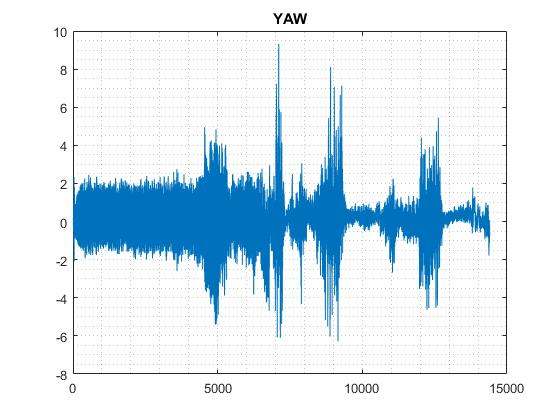
\includegraphics[width = 0.6\textwidth]{VAPIQ-PICTURES/YAWshaftTrow.jpg}
      \caption{Gyroscope yaw raw data}
    \label{fig:yo}
\end{figure} 
Fig. \ref{fig:PIKK2} shows the mounting of the IMU. 
\begin{figure}[H]
    \centering
         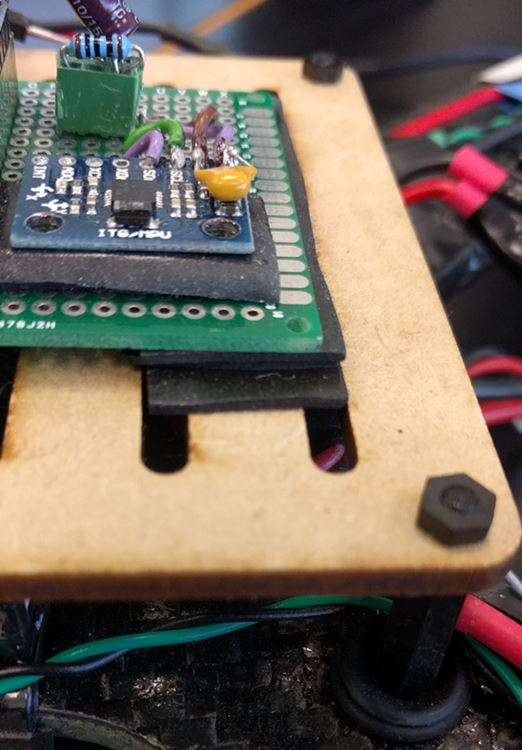
\includegraphics[width = 0.2\textwidth]{VAPIQ-PICTURES/SensorDritt.jpg}
      \caption{IMU mount}
    \label{fig:PIKK2}
\end{figure} 
To reduce vibrations the IMU and prototype board is mounted with double sided tape, see Fig. \ref{fig:PIKK2}. The upper plate of the quadcopter is placed on nylon standoffs with rubber gaskets underneath. The IMU sensor has holes which allows for fastening with screws. The IMU has been fastened with screws, and the result was more vibrations. The vibrations got worse because of the fasteners carrying the vibrations from the frame to the sensor. \bigskip

The vibrations in the frame becomes severe when the RPM of the motor matches the mechanical resonance frequency of the frame. The resonance frequency appears at approximately 10 600 RPM . Plywood pieces have been mounted to the arms of the frame to give extra stiffness. This has improved the problem with mechanical resonance frequencies and allows for higher RPM´s. It was also observed that the vibrations got better when the motors were operating on overcritical RPM´s.
%%%%%%%%%%%%%%%%%%%%%%%%%%%%%%%%%%%%
%%%%%%%%%%%%%%%%%%%%%%%%%%%%%%%%%%%%
\section{Electrical Counter Measures}
The IMU is exposed to electrical noise. The noise can be caused by any electronic device or by voltage fluctuations.\bigskip

To minimize the problem with voltage fluctuations a capacitor of 100nF has been placed between Vcc and GND on the IMU to smooth the voltage. An analog RC low-pass filter has also been added to suppress high frequency noise. The RC low-pass filter has a cutoff frequency of
\begin{equation}
    F_c = \frac{1}{2\pi RC} = \frac{1}{2\pi 100\Omega (100nF + 4.7\mu F)} = 330 Hz. 
\end{equation}
The filter implementation gave a significant improvement to the readings from the IMU. 
\begin{figure}[H]
    \centering
         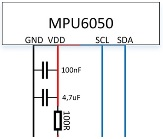
\includegraphics[width = 0.2\textwidth]{VAPIQ-PICTURES/Sensor.jpg}
      \caption{IMU circuit}
    \label{fig:PIKK}
\end{figure} 
The quadrotor has several sources that induce noise on the IMU. The ESCs for example, produces noise which can easily be picked up by the IMU. To reduce the effects of electrical noise, the cables must be shortened to a minimum. To ensure minimum electrical interference, the IMU should be placed far away from components that can cause disturbances. 

\section{Software Counter Measures}
If the quadrotor is optimized mechanically and electrically against vibrations and noise, the rest must be taken care of in software by means of filtering. There are several filters that are possible to implement. The biggest concern when choosing a filter is the delay and the computational complexity.\bigskip

Several methods have been considered and tested:
\begin{itemize}
    \item FIR low-pass filter
    \item IIR notch filter
    \item Running average
    \item Complementary filter  % write short about
    \item Kalman filter         % Wrrte short about
\end{itemize}
Choosing the appropriate processing method is always a trade-off between computational complexity, the number of samples and the ability to suppress frequency components. Increasing the number of samples yields a better ability to suppress noise. The main loop of the flight controller is running at 250 Hz which limits the number of samples available for processing. The gyro can be sampled up to 8kHz and the accelerometer can be sampled up to 1kHz i.e. the maximum number of samples that can be used for processing is 32 and 4 respectively.
\begin{figure}[H]
%\label{fig:rawData}
        \centering
            \begin{minipage}[b]{0.32\textwidth}
                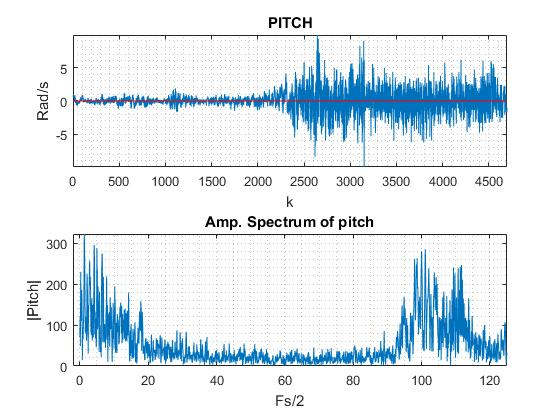
\includegraphics[width = \textwidth, angle= 0]{VAPIQ-PICTURES/PITCH1.jpg}
                \caption{Pitch}
                    \label{fig:Pitch}
            \end{minipage}
            \hfill
            \begin{minipage}[b]{0.32\textwidth}
                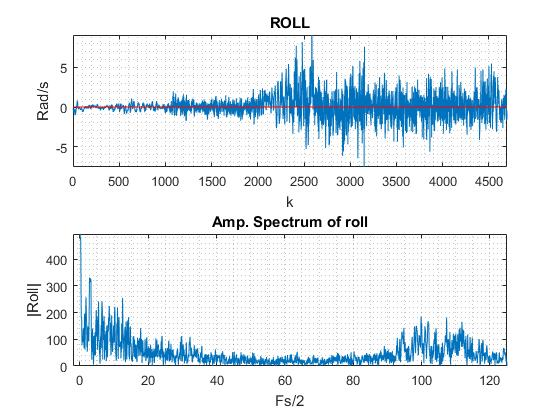
\includegraphics[width =\textwidth, angle =0]{VAPIQ-PICTURES/ROLL1.jpg}
                \caption{Roll}
                \label{fig:Roll}
            \end{minipage}
            \hfill
            \begin{minipage}[b]{0.32\textwidth}
                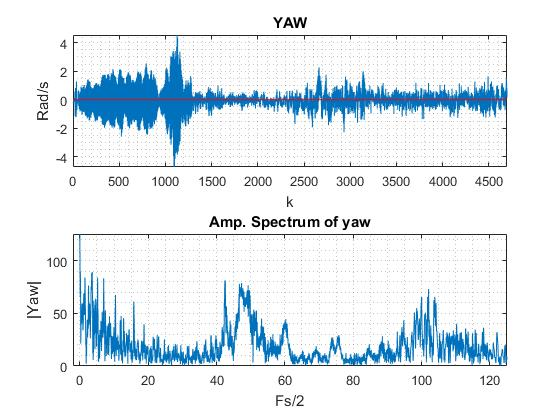
\includegraphics[width =\textwidth, angle =0]{VAPIQ-PICTURES/YAW1.jpg}
                \caption{Yaw}
                \label{fig:Yaw}
            \end{minipage}
%\caption{Raw gyroscope data}
\end{figure}
Fig. \ref{fig:Pitch}, \ref{fig:Roll} \& \ref{fig:Yaw} shows the raw data from the gyroscope. The quadcopter is initially at rest on a flat table and the thrust is slowly increased. The figures shows the data in the time domain at the top, and in the frequency domain at the bottom. The time domain plots show that the gyroscope gets inaccurate when the thrust is approximately 50 \%. Roll and pitch is off by $\pm$ 10 deg/s at worst, yaw is of by $\pm$ 6 deg/s. The data seems to be symmetric around the origin, which implies that averaging the data will effectively reduce the noise. \bigskip 

A moving average filter is a causal filter i.e. it uses only present and past values to compute the output. Since no future values is used this filter works in real time. Equation \ref{MovAvg} describes a 3-point moving average filter. This filter has low pass characteristics and is used to smooth out the data.
\begin{equation}
    \label{MovAvg}
    y[n] = \frac{1}{3}(x[n] + x[n-1] + x[n-2])
\end{equation}

Fig. \ref{MovAvg} shows the data from Fig. \ref{fig:Roll} with applied moving average filter.
This sequence uses 10 samples to compute the mean. 
\begin{figure}[H]
    \centering
         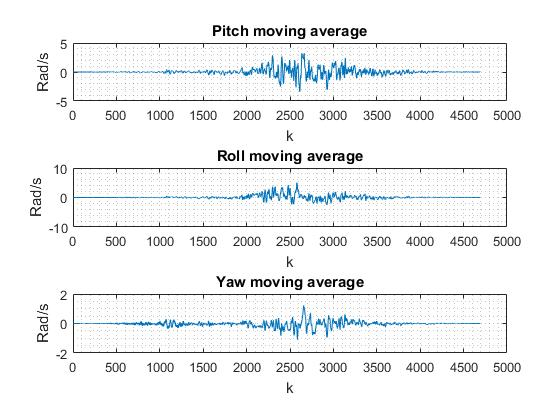
\includegraphics[width = 0.6\textwidth]{VAPIQ-PICTURES/MovingAverageFigure.jpg}
      \caption{Moving average}
    \label{fig:MovAvg}
\end{figure} 
This figure shows that a moving average filter will improve the gyro values up to around 50-60\% thrust. At thrust levels above these values, the vibrations will become so severe that the filter cannot remove the noise. 
\begin{figure}[H]
        \centering
            \begin{minipage}[b]{0.49\textwidth}
                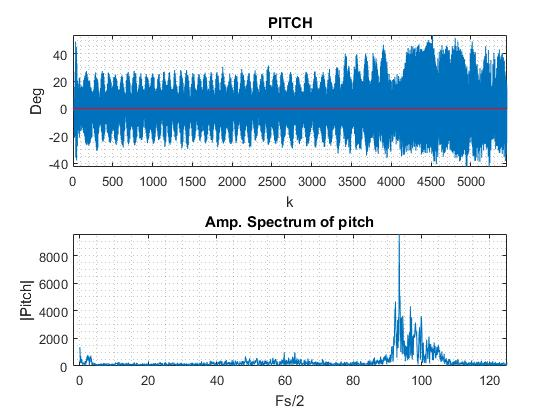
\includegraphics[width = \textwidth, angle= 0]{VAPIQ-PICTURES/PITCHacc.jpg}
                \caption{Pitch Accelerometer}
                \label{fig:PitchAcc}
            \end{minipage}
            \hfill
            \begin{minipage}[b]{0.49\textwidth}
                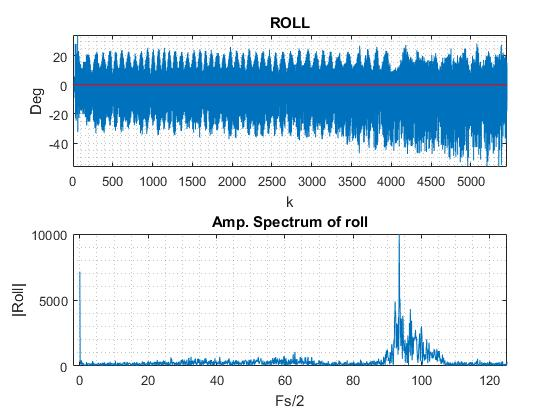
\includegraphics[width =\textwidth, angle =0]{VAPIQ-PICTURES/ROLLacc.jpg}
                \caption{Roll Accelerometer}
                \label{fig:RollAcc}
            \end{minipage}
%\label{fig:rawDataAcc}
\caption{Raw Accelerometer Data}
\end{figure}
Fig. \ref{fig:PitchAcc} \& \ref{fig:RollAcc} shows the raw accelerometer data. This data is also obtained from when the quadrotor is initially at rest on a flat table and until thrust reaches the maximum. The data is observed to be noisy and needs to be processed in order to be usable. The amplitude spectrum of the data, shows that most of the noise is in the frequency area of 100 Hz. This noise can be filtered with a IIR Notch filter.
\begin{figure}[H]
    \centering
         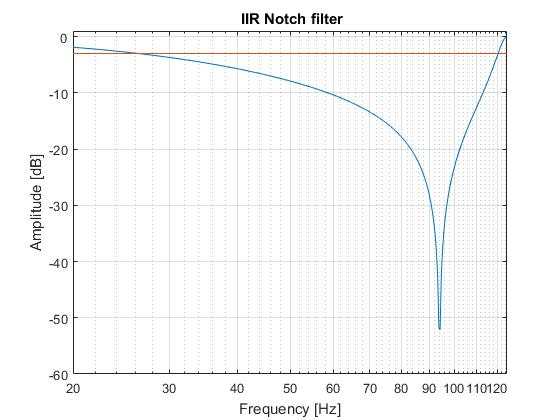
\includegraphics[width = 0.6\textwidth]{VAPIQ-PICTURES/NotchResp.jpg}
      \caption{Notch Filter}
    \label{fig:notchResp}
\end{figure} 
The frequency response of the notch filter is seen in figure \ref{fig:notchResp}. The filter is designed to remove the dominant frequency components around 90-100 Hz.
% Skriv kort om specc til notch filter
\begin{figure}[H]
    \centering
         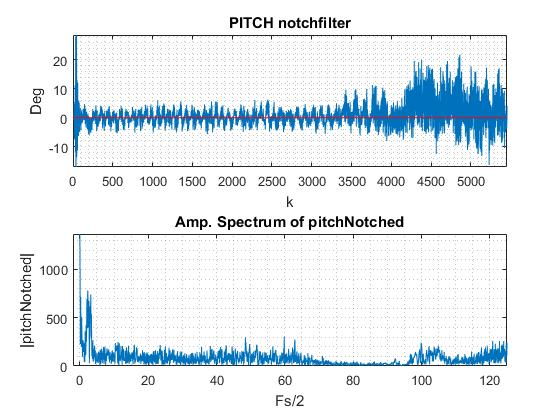
\includegraphics[width = 0.6\textwidth]{VAPIQ-PICTURES/PitchNotchFilt.jpg}
      \caption{Moving average}
    \label{fig:pitchNotchedFig}
\end{figure}
Applying the notch filter to the data sequence yields Fig. \ref{fig:pitchNotchedFig}. \bigskip

The data got significantly better when using the notch filter, but there is still noise. The frequency spectrum shows that there are many frequency components distributed throughout the entire spectrum. Implementing a FIR LP filter will probably yield a better result than using the notch filter. Many notch filters are probably required if this approach shall work. Therefore, a FIR LP filter will require less computational power. \bigskip

The FIR filter is implemented in direct form, seen in Fig. \ref{fig:directForm}.
\begin{figure}[H]
    \centering
         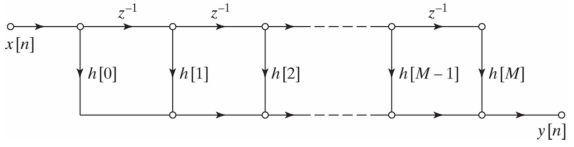
\includegraphics[width = 0.5\textwidth]{VAPIQ-PICTURES/DirectFormImplementation.jpg}
      \caption{Direct form implementation}
    \label{fig:directForm}
\end{figure}
\begin{equation}
    y[n] = \sum_{k = 0}^{M} h[k]x[n-k]
    \label{Convolution}
\end{equation}
Equation \ref{Convolution} describes the output of the FIR filter seen in figure \ref{fig:directForm}. x[n] represents the input sequence which is convolved with the filter coefficients h[n]. K represents every delay step in the filter. The following code snippet implements the FIR LP in C\#/C++.
\begin{lstlisting}[frame=single]  % Start your code-block
int i = 0;
  for(i=N; i>0; i--) {  // Shiftregister:
      x[i] = x[i-1];    // Shifts all previous samples one position
      y[i] = y[i-1];
      z[i] = z[i-1];
  }

  x[0] = acc_x;         // Receive newest sample into shiftregister
  y[0] = acc_y;
  z[0] = acc_z;

  acc_x = h[0] * x[0];       // Compute the convolution x[0]*h[0]
  acc_y = h[0] * y[0];
  acc_z = h[0] * z[0];
 
  for(i = 1; i <= N; i++) {  // Convolve rest of the inputs
    acc_x += h[i] * x[i];    // with the filter coefficients
    acc_y += h[i] * y[i];
    acc_z += h[i] * z[i];
  }
\end{lstlisting}
Fig. \ref{fig:FIRlpFilter} shows the frequency response of the FIR LP filter. The filter has a cutoff frequency of 6 Hz and a attenuation of 54 dB with an order of 22. An order of 22 gives a total delay of 21 samples i.e. the total delay is (N-1)$T_s$ = (N-1)$\frac{1}{F_s}$ = 21$\frac{1}{250Hz}$ = 0.1s.
\begin{figure}[H]
        \centering
            \begin{minipage}[b]{0.45\textwidth}
                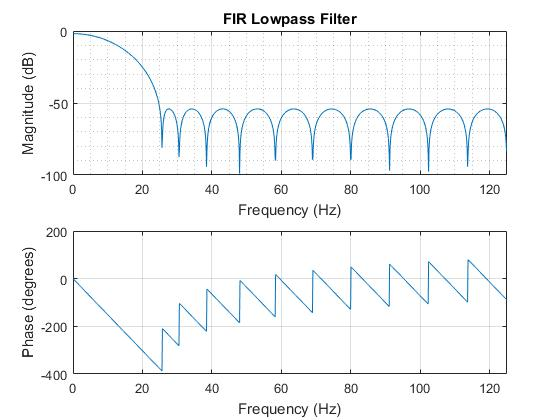
\includegraphics[width = \textwidth, angle= 0]{VAPIQ-PICTURES/FIRlowPASSfilter.jpg}
                \caption{FIR LP filter}
                    \label{fig:FIRlpFilter}
            \end{minipage}
            \hfill
            \begin{minipage}[b]{0.45\textwidth}
                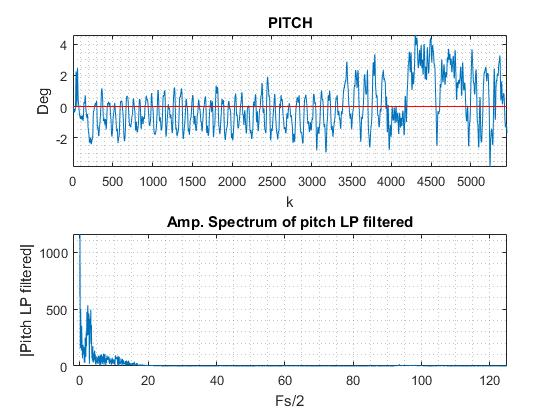
\includegraphics[width =\textwidth, angle =0]{VAPIQ-PICTURES/PitchAccelometerLPFiltered.jpg}
                \caption{Pitch accelometer LP filtered}
                \label{fig:pitchLPfiltered}
            \end{minipage}
\end{figure}
Fig. \ref{fig:pitchLPfiltered} shows the filtered accelerometer data for pitch. The angle is off by approximately 2 degrees, which is a better result than for the notch filter. \bigskip

The gyroscope is prone to drift over time, but very precise in a short time span.  The accelerometer is very sensitive to vibrations and therefore very imprecise for short timespan, but it does not have any drift. For this reason the IMU will output wrong angles. A solution to this is to use the well know Kalman Filter. This filter merges both sensors to obtain the 

\section{Conclusion}
There has been several challenges regarding vibrations and noise on the quadrotor. Mechanical vibrations is the greatest limitation to the performance of the quadrotor. The vibrations increases significantly when variable pitch is introduced. The trust is limited to 50-60\% for this reason. Several methods of filtering have been tested on the IMU data. In the flight controller, a moving average filter is applied to the gyro values. The gyro will output perfect data up to approximately 50-60\% thrust, this is where the vibrations gets to excessive. The accelerometer is much more prone to vibrations than the gyro and needs more processing. A FIR LP filter makes the accelerometer values acceptable. 



%%Resonance frequecies in frame